\part{Basic Content in LaTeX{}}

\section{\LaTeX{}'s Interpretation of Plain Text}

\begin{itemize}
\item The entire \texttt{.tex} file you write will contain only characters on
  your keyboard. That means, somehow, the characters on your keyboard you need
  to represent: a, A, $\alpha$, $\mathbb{A}$, \`a, \texttt{A}, $_a$, and \"A.

\item The file that you write will be composed entirely of the characters in
  Table~\ref{tab:chars}. This is true no matter what kind of crazy symbols are
  ultimately included, such as \staveVI.

  \begin{table}[h]
    \centering
    \begin{center}
      \begin{minipage}{.85\textwidth}
        \begin{framed}
\begin{verbatim}
a b c d e f g h i j k l m n o p q r s t u v w x y z
A B C D E F G H I J K L M N O P Q R S T U V W X Y Z
0 1 2 3 4  6 7 8 9
! @ # $ % ^ & * ( ) _ +
{ } [ ] | \ l ; : ' " < , > . ? /
\end{verbatim}
        \end{framed}
      \end{minipage}
    \end{center}
    \caption{Characters To Use in \texttt{.tex} Files} \label{tab:chars}
  \end{table}
\end{itemize}

\subsection*{Special Characters}

\begin{itemize}

\item The following characters are reserved or \textit{special}:

  \begin{table}[h]
    \centering
    \begin{center}
      \begin{minipage}{.5\textwidth}
        \begin{framed}
\begin{verbatim}
% # $ ^ & _ { } ~ \
\end{verbatim}
        \end{framed}
      \end{minipage}
    \end{center}
    \caption{Special Characters in \texttt{.tex} Files} \label{tab:spec}
  \end{table}

\item By special, we mean that each of these characters in the \LaTeX{} file
  doesn't represent itself in your output file. If you type ``\texttt{\%}'' into
  your text editor and build your output, you will not get a percent
  sign. Rather, these \textit{special} characters mean something very specific
  to \LaTeX{}.

\item In order to generate these symbols in your \textit{output} you need to use
  other, non-literal representations.

  Although detailed descriptions of these symbols is beyond
  the purpose of this section, accept the following brief comments:\\

  \begin{table}[h]
    \centering
    \begin{framed}
      \begin{tabular}[h]{r p{3.5in}}
        \textbf{Character} & \textbf{Purpose} \\
        \hline
        \texttt{\%} & used for including comments and preventing \LaTeX ~from interpreting file contents \\
        \texttt{\#} & used to define \LaTeX{} commands (or macros) \\
        \texttt{\$} & used to start \LaTeX{} math mode \\
        \texttt{\textasciicircum{}} & used for superscripts in math mode \\
        \texttt{\_} & used for subscripts in math mode \\
        \texttt{\&} & used for alignment in \LaTeX{} math and tables \\
        \texttt{\{ \}} & used to pass arguments to \LaTeX{} commands \\
        \texttt{\~{}} & used to represent a special kind of whitespace \\
        \texttt{\textbackslash} & used to start every \LaTeX{} command \\
      \end{tabular}
    \end{framed}

    \caption{Purpose of Special Characters}
  \end{table}

\end{itemize}

\subsection*{Commands}

\begin{itemize}

\item \par Using \LaTeX{} efficiently often requires one be familiar with
  various \LaTeX commands (or macros). In general, this comes only with
  practice. Commands start with a ``\texttt{\textbackslash}'' and they are
  case-sensitive. Commands can be used to generate particular glyphs (think
  shapes on the page) or alter the content in some way.

\item \par One command is ``\texttt{\textbackslash LaTeX\{\}}'' which
  produces ``\LaTeX''. Similarly, ``\texttt{\textbackslash
    textbf\{election\}}'' produces ``\textbf{election}''.

\item \par You'll never learn a significant proportion of all the \LaTeX~
  commands that people use. However, you'll eventually memorize the ones
  you use over and over and know how to look up the rest.

\item \par The mandatory arguments to a command are passed inside curly braces
  and the option arguments to a macro are passed inside square brackets. The
  result is something like
\begin{verbatim}
\command[optional1=1, optional2=2]{mandatory=Always}
\end{verbatim}
  where the (optional) argument \texttt{optional1} is being passed the value 1,
  the (optional) argument \texttt{optional2} is being passed the value 2, and
  the (mandatory) argument \texttt{mandatory} is passed the value ``Always''.
\end{itemize}

\subsection*{Whitespace and Spacing}

\begin{itemize}

\item 2 or more carriage returns, ``\texttt{\textbackslash\textbackslash}'', and
  ``\texttt{\textbackslash linebreak}'' break lines

\item ``\texttt{\~}'' is a non-breaking space

\item ``\verb=\par='' will create a new paragraph for the
  succeeding text, regardless of surrounding whitespace

\item ``\verb=\linebreak='' and ``\verb=\pagebreak='' are appropriately
  named

\item multiple consecutive spaces are interpreted as one
\end{itemize}

So, \\

\lstinputlisting{./chapters/02_basic/sounds}

produces the following text:

\begin{framed}
  \begin{minipage}{.5\textwidth}
  And in the naked light I saw \\ Ten thousand people, maybe more.

      People talking without speaking, \\
      People~hearing~without~listening,

People writing
songs that voices never share \par And no one dared

Disturb      the        sound        of       silence.
  \end{minipage}
\end{framed}


\section{\texttt{.tex} Input File Structure}

\begin{itemize}

\item \LaTeX{} \texttt{.tex} files have a particular structure. If the file you
  attempt to compile has an error, your document will either fail to be produced
  or it will not be compiled in accordance with your intentions.

\item First, you must declare the \textit{document class}: \\


  \begin{center}
    \begin{minipage}{.8\linewidth}
      \begin{framed}
\begin{verbatim}
\documentclass[letterpaper, 10pt]{article}
\end{verbatim}
      \end{framed}
    \end{minipage}
  \end{center}
  or \\

  \begin{center}
    \begin{minipage}{.8\linewidth}
      \begin{framed}
\begin{verbatim}
\documentclass[12pt]{letter}
\end{verbatim}
      \end{framed}
    \end{minipage}
  \end{center}

  and this is part of the \textit{preamble}. For most purposes,
  \texttt{article} is sufficient.

\item \par Second, the remainder of the preamble contains explicit calls to
  outside packages if you require their functionality, the creation of
  new macros, and setting document properties. After the
  \texttt{\textbackslash documentclass} command we might see the
  following lines:\\

  \begin{center}
    \begin{minipage}{.8\linewidth}
      \begin{framed}
\begin{verbatim}
\usepackage{fancyhdr}

\pagestyle{fancy}
\cfoot{\thepage}
\title{A Document}
\end{verbatim}
      \end{framed}
    \end{minipage}
  \end{center}

  which provides the functionality from the \texttt{fancyhdr} package, sets the
  ``\texttt{pagestyle}'' to ``fancy'', places the page number in the center of
  the footer, and sets the title to ``A Document''.

  This is also part of the \textit{preamble}.

\item Third, the main content is typed within the ``\texttt{document}''
  environment, as in: \\

  \begin{center}
    \begin{minipage}{.8\linewidth}
      \begin{framed}
\begin{verbatim}
\begin{document}

%% place content here

\end{document}
\end{verbatim}
      \end{framed}
    \end{minipage}
  \end{center}

\item Lastly, any characters occurring after the close of the \texttt{document}
  environment will be ignored by \LaTeX{}. This includes special characters and
  commands.

\end{itemize}

In its entirety, we might have the following \texttt{.tex} file:

\lstinputlisting[caption=\texttt{fakefile2.tex}]{./chapters/02_basic/fakefile2.tex}

\begin{figure}[h]
  \centering
  \fbox{
    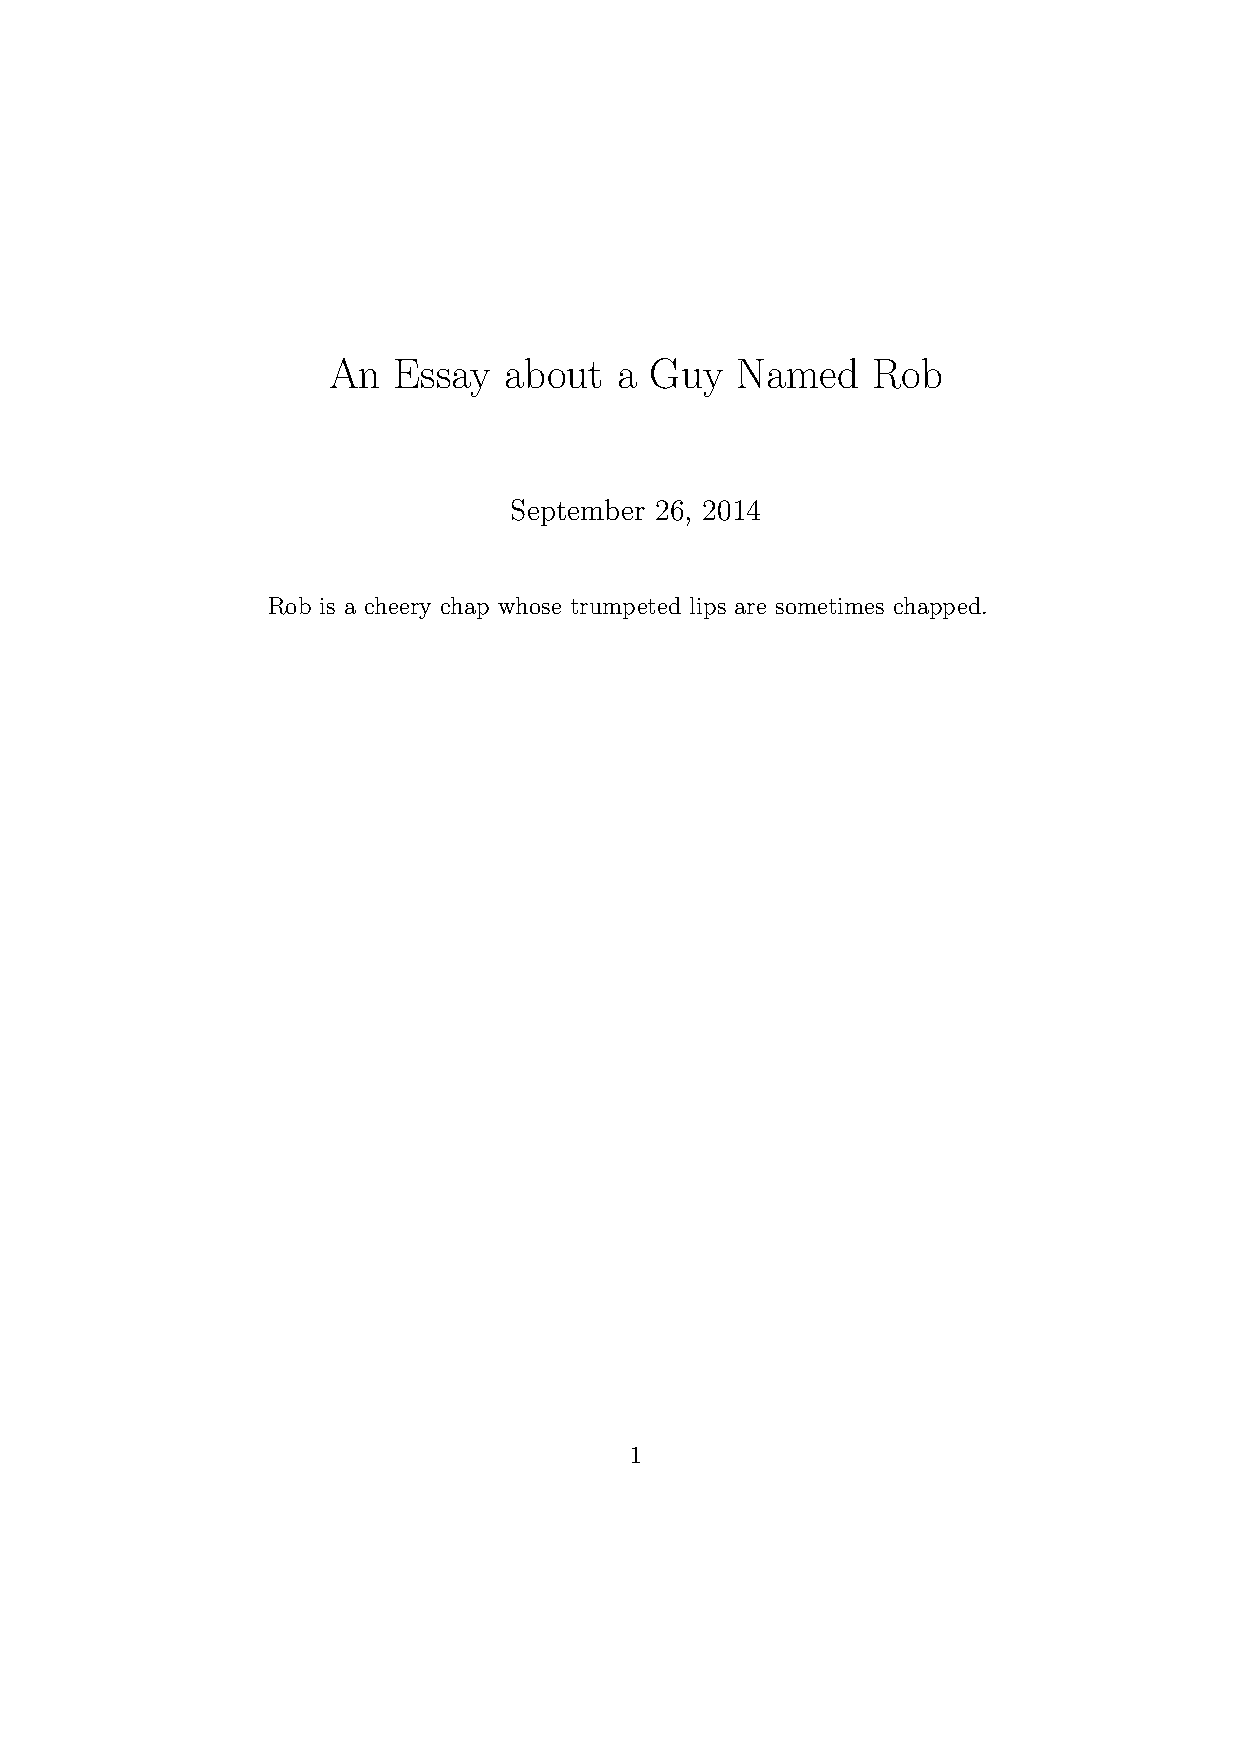
\includegraphics[scale=.4]{./chapters/02_basic/fakefile2}
  }
  \caption{Output from Example Input: \texttt{fakefile2.tex}}
\end{figure}

\marginpar{Go ahead and compile this document after you type it out.}

\clearpage

\section{Output File Structure}
\subsection*{Headings}

\begin{itemize}
\item \LaTeX~accepts the definition of a document hierarchy and displays
  headings appropriately. The \textit{article} class accepts the following
  headings whose order indicates how far down they are in the order:
  \texttt{\textbackslash part\{\}}, \texttt{\textbackslash section\{\}},
  \texttt{\textbackslash subsection\{\}}, \texttt{\textbackslash
    subsubsection\{\}}, \texttt{\textbackslash paragraph\{\}}, and
  \texttt{\textbackslash subparagraph\{\}}. If an ``\texttt{*}'' is placed after
  the name as in ``\texttt{\textbackslash part*\{\}}'' then the heading will not
  be numbered and will not be included in the table of contents, if it
  exists. Otherwise it will be numbered and included in the table of
  contents. The one mandatory argument is the text of the heading.

\item Any headings after the \verb=\appendix= command will be altered to reflect
  that they do not belong to the main body of the text and, rather, the
  appendix.

  \marginpar{Add a \texttt{section} and a \texttt{subsection*} heading to your
    document. Name them after your two favorite colors. Compile the document.}

\end{itemize}

\section{Environments}

\begin{itemize}
\item All of the content that will be displayed in your final document is
  contained in at least one environment. Environments are contexts which affect
  how the content is rendered and interpreted. Environments are indicated by the
  \verb=\begin{env}= and \verb=\end{env}= commands. We have already seen the
  \texttt{document} environment.

\item We will discuss various environments (and there are many) during the
  remainder of the week, but the basics are all the same. If you begin
  an environment, you must end it. When nesting environments, the most
  recently opened environment must be closed before an earlier
  environment can be closed.

\item The \texttt{enumerate} environment creates ordered lists. The
  \texttt{itemize} environment creates unordered lists. The
  \texttt{table} environment is used to encapsulate table-like content.

  \marginpar{At the end of your content begin and end a ``tiny''
    environment. Inside this environment type your favorite thing to shout. Use
    proper latex quotes (\textit{i.e.}\ ``\ldots '' and not
    "\ldots"). Compile the document.}

The insertion might look like

\begin{center}
  \begin{minipage}{.8\linewidth}
    \begin{framed}
\begin{verbatim}
\begin{tiny}
``Stellaaaaaaaaa!''
\end{tiny}
\end{verbatim}
    \end{framed}
  \end{minipage}
\end{center}

\end{itemize}

\section{Error Debugging}

You will, invariably, make errors. However, you'll probably never be
the first person to make any particular error. The four most common
errors are
\begin{enumerate}
\item you type a command incorrectly

\item you forget to \verb=\usepackage= the package that supplies a command which
  \LaTeX{} interprets as if you typed a command incorrectly

\item you don't \verb=\end{env}= what you \verb=\begin{env}= or you abuse the
  order of nested environments

\item you have un-balanced braces/parenthesis/brackets depending on
  what \LaTeX{} is looking for.

\end{enumerate}

Place the \texttt{tiny} environment inside a \texttt{center}
  environment. Now, change one of the \verb=\begin= commands to
    \verb=\benign=. Compile it. This is not benign! Look at the error
    message. Correct this mistake and swap the two \texttt{end}
    statements. Compile the document now. Look at the error message.


\section{Solving Problems and Getting Help}

\begin{itemize}
\item Don't panic.
\item Check the usual suspects.
\item Google a description of your problem in addition to ``latex
  ctan.'' Including ``latex'' without ``ctan'' is a bad, bad, bad,
  bad, bad idea!
\item Comment out potential sources of the problem until you
  identify it. Slowly add things back in until you have removed only
  the offending portion. Can this be fixed?

%% \item Consult one of the \LaTeX~ books in the star lab.

\item Consult one of the many great \LaTeX~sites out there.\footnote{Google
    either ``latex ctan wikibook'' or ``latex comprehensive symbol''. These two
    are great.}

\item Ask a friend!

%% \item Ask the star lab fellow!

\end{itemize}

%%% Local Variables:
%%% mode: latex
%%% TeX-master: "../../tutorial"
%%% End:
